%Este trabalho está licenciado sob a Licença Atribuição-CompartilhaIgual 4.0 Internacional Creative Commons. Para visualizar uma cópia desta licença, visite http://creativecommons.org/licenses/by-sa/4.0/deed.pt_BR ou mande uma carta para Creative Commons, PO Box 1866, Mountain View, CA 94042, USA.

\documentclass[12pt]{book}

\input ../preambulo.tex

\ifispython
\lstset { %
  language=Python,
}
\fi

\makeindex

\begin{document}

\frontmatter

\title{Redes Neurais Artificiais}
\author{Pedro H A Konzen}
\date{\today}
\ifishtml
\else
\addcontentsline{toc}{chapter}{Capa}
\fi

\maketitle

\nocite{Goodfellow2016a}

%Este trabalho está licenciado sob a Licença Atribuição-CompartilhaIgual 4.0 Internacional Creative Commons. Para visualizar uma cópia desta licença, visite http://creativecommons.org/licenses/by-sa/4.0/ ou mande uma carta para Creative Commons, PO Box 1866, Mountain View, CA 94042, USA.

\chapter*{Licença}\label{licenca}
\addcontentsline{toc}{chapter}{Licença}

Este trabalho está licenciado sob a Licença Atribuição-CompartilhaIgual 4.0 Internacional Creative Commons. Para visualizar uma cópia desta licença, visite http://creativecommons.org/licenses/by-sa/4.0/deed.pt\_BR ou mande uma carta para Creative Commons, PO Box 1866, Mountain View, CA 94042, USA.

%Este trabalho está licenciado sob a Licença Atribuição-CompartilhaIgual 4.0 Internacional Creative Commons. Para visualizar uma cópia desta licença, visite http://creativecommons.org/licenses/by-sa/4.0/deed.pt_BR ou mande uma carta para Creative Commons, PO Box 1866, Mountain View, CA 94042, USA.

\chapter*{Prefácio}\label{prefacio}
\addcontentsline{toc}{chapter}{Prefácio}

O site \href{https://www.notaspedrok.com.br}{notaspedrok.com.br} é uma plataforma que construí para o compartilhamento de minhas notas de aula. Essas anotações feitas como preparação de aulas é uma prática comum de professoras/es. Muitas vezes feitas a rabiscos em rascunhos com validade tão curta quanto o momento em que são concebidas, outras vezes, com capricho de um diário guardado a sete chaves. Notas de aula também são feitas por estudantes - são anotações, fotos, prints, entre outras formas de registros de partes dessas mesmas aulas. Essa dispersão de material didático sempre me intrigou e foi o que me motivou a iniciar o site.

Com início em 2018, o site contava com apenas três notas incipientes. De lá para cá, conforme fui expandido e revisando os materais, o site foi ganhando acessos de vários locais do mundo, em especial, de países de língua portugusa. No momento, conta com 13 notas de aula, além de minicursos e uma coleção de vídeos e áudios.

As notas de \emph{Redes Neurais Artificiais} fazem uma introdução às redes neuraus artificiais com enfase na resolução de problemas de matemática. Como ferramenta de apoio computacional, códigos exemplos são trabalhos em linguagem {\python}, mais especificamente, com o pacote de aprendizagem de máquina {\pytorch}.

Aproveito para agradecer a todas/os que de forma assídua ou esporádica contribuem com correções, sugestões e críticas! ;)

\begin{flushright}
  Pedro H A Konzen

  \url{https://www.notaspedrok.com.br}
\end{flushright}



\tableofcontents
\addcontentsline{toc}{chapter}{Sumário}

\mainmatter

%Este trabalho está licenciado sob a Licença Atribuição-CompartilhaIgual 4.0 Internacional Creative Commons. Para visualizar uma cópia desta licença, visite http://creativecommons.org/licenses/by-sa/4.0/deed.pt_BR ou mande uma carta para Creative Commons, PO Box 1866, Mountain View, CA 94042, USA.

\chapter{Introdução}\label{cap_intro}
\thispagestyle{fancy}

\begin{flushright}
  [Vídeo] | [Áudio] | \href{https://phkonzen.github.io/notas/contato.html}{[Contatar]}
\end{flushright}

\emconstrucao

%Este trabalho está licenciado sob a Licença Atribuição-CompartilhaIgual 4.0 Internacional Creative Commons. Para visualizar uma cópia desta licença, visite http://creativecommons.org/licenses/by-sa/4.0/deed.pt_BR ou mande uma carta para Creative Commons, PO Box 1866, Mountain View, CA 94042, USA.

\chapter{Perceptron}\label{cap_perceptron}
\thispagestyle{fancy}
[[tag:construcao]]


\section{Unidade de Processamento}\label{cap_perceptron_sec_unit}
[[tag:construcao]]

A \hl{\emph{unidade básica de processamento}} (neurônio artificial) que exploramos nestas notas \hl{é baseada no \emph{perceptron}} (consultemos a Fig. \ref{fig:perceptron}). \hl{Consiste na composição de uma \emph{função de ativação} $f:\mathbb{R}\to\mathbb{R}$ com a \emph{pré-ativação}}
\begin{align}
  \hleq{z} &\hleq{= \pmb{w}\cdot\pmb{x} + b} \\
    &= w_1x_1 + w_2x_2 + \cdots + w_nx_n + b
\end{align}
onde, $\pmb{x}\in\mathbb{R}^{n}$ é o \emph{vetor de entrada}, $\pmb{w}\in\mathbb{R}^{n}$ é o \emph{vetor de pesos} e $b\in\mathbb{R}$ é o \emph{\textit{bias}}. Escolhida uma função de ativação, a \emph{saída do neurônio} é dada por
\begin{align}
  \hleq y &\hleq := \mathcal{N}\left(\pmb{x};(\pmb{w},b)\right)\\
    &= f(z) = f(\pmb{w}\cdot\pmb{x} + b)
\end{align}
\hl{O treinamento (calibração) consiste em determinar os parâmetros $(\pmb{w}, b)$ de forma que o neurônio forneça as saídas $y$ esperadas com base em algum critério predeterminado}.

\begin{figure}[H]
  \centering
  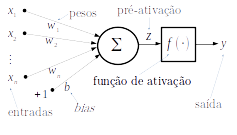
\includegraphics[width=0.7\textwidth]{./cap_perceptron/dados/fig_perceptron/fig}
  \caption{Esquema de um perceptron: unidade de processamento.}
  \label{fig:perceptron}
\end{figure}

Uma das vantagens deste modelo de neurônio é sua generalidade, i.e. pode ser aplicado a diferentes problemas. Na sequência, vamos aplicá-lo na resolução de um problema de classificação e noutro de regressão.


\subsection{Um problema de classificação}\label{cap_perceptron_ssec_classic}
[[tag:construcao]]

\hl{Vamos desenvolver um perceptron que emule a operação $\land$ (e-lógico)}. I.e, receba como entrada dois valores lógicos $A_1$ e $A_2$ (V, verdadeiro ou F, falso) e forneça como saída o valor lógico $R = A_1 \land A_2$. Consultamos a seguinte tabela verdade:

\begin{center}
  \begin{tabular}{cc|c}
    $A_1$ & $A_2$ & R\\\hline
    V & V & V\\
    V & F & F\\
    F & V & F\\
    F & F & F\\\hline
  \end{tabular}
\end{center}


\subsubsection{Modelo}
[[tag:construcao]]

Nosso \hl{\emph{modelo de neurônio}} será \hl{um perceptron com duas entradas $\pmb{x}\in \{-1,1\}^2$} e a função sinal
\begin{equation}
  f(z) = \sign(z) = \left\{
    \begin{array}{rr}
      1 &, z>0\\
      0 &, z=0\\
      -1 &, z<0
    \end{array}
\right.
\end{equation}
como função de ativação, i.e.
\begin{equation}
  \mathcal{N}\left(\pmb{x};(\pmb{w},b)\right) = \sign(\pmb{w}\cdot\pmb{x} + b),
\end{equation}
onde $\pmb{w}\in\mathbb{R}^2$ e $b\in\mathbb{R}$ são parâmetros a determinar.


\subsubsection{Pré-processamento}
[[tag:construcao]]

Uma vez que nosso modelo recebe valores $\pmb{x}\in \{-1,1\}^2$ e retorna $y\in\{-1,1\}$, precisamos (pre)processar os dados do problema de forma a utilizá-lo. Uma forma, é assumir que todo valor negativo está associado ao valor lógico $F$ (falso) e positivo ao valor lógico $V$ (verdadeiro). Desta forma, os dados podem ser interpretados como na tabela abaixo.

\begin{center}
  \begin{tabular}{rr|c}
    $x_1$ & $x_2$ & $y$\\\hline
    1 & 1 & 1\\
    1 & -1 & -1\\
    -1 & 1 & -1\\
    -1 & -1 & -1\\\hline
  \end{tabular}
\end{center}
    
    
\subsubsection{Treinamento}
[[tag:construcao]]

Agora, nos falta \hl{treinar nosso neurônio para fornecer o valor de $y$ esperado para cada dada entrada $\pmb{x}$}. Isso \hl{consiste em um método para escolhermos os parâmetros $(\pmb{w},b)$} que sejam adequados para esta tarefa. Vamos explorar mais sobre isso na sequência do texto e, aqui, apenas escolhemos
\begin{gather}
  \pmb{w} = [1, 1]\\
  b = -1
\end{gather}
Com isso, nosso perceptron é
\begin{equation}
  \mathcal{N}(\pmb{x}) = \sign(x_1 + x_2 - 1)
\end{equation}
Verifique que ele satisfaz a tabela verdade acima!


\subsubsection{Implementação}
[[tag:construcao]]

% {./cap_perceptron/dados/py_perceptron/main.py}
\begin{lstlisting}[caption=perceptron.py, label=cap_perceptron_sec_unit:cod:perceptron]
import torch

# modelo
class Perceptron(torch.nn.Module):
    def __init__(self):
        super().__init__()
        self.linear = torch.nn.Linear(2,1)

    def forward(self, x):
        z =  self.linear(x)
        y = torch.sign(z)
        return y

model = Perceptron()
W = torch.Tensor([[1., 1.]])
b = torch.Tensor([-1.])
with torch.no_grad():
    model.linear.weight = torch.nn.Parameter(W)
    model.linear.bias = torch.nn.Parameter(b)

# dados de entrada
X = torch.tensor([[1., 1.],
                  [1., -1.],
                  [-1., 1.],
                  [-1., -1.]])

print(f"\nDados de entrada\n{X}")


# forward (aplicação do modelo)
y = model(X)

print(f"Valores estimados\n{y}")
\end{lstlisting}

\subsubsection{Interpretação geométrica}
[[tag:construcao]]

Empregamos o seguinte modelo de neurônio
\begin{equation}
  \mathcal{N}\left(\pmb{x};(\pmb{w},b)\right) = \sign(w_1x_1 + w_2x_2 + b)
\end{equation}
Observamos que
\begin{equation}
  w_1x_1 + w_2x_2 + b = 0
\end{equation}
corresponde à equação geral de uma reta no plano $\tau: x_1\times x_2$. Esta reta divide o plano em dois semiplanos
\begin{align}
  \tau^+ = \{\pmb{x}\in\mathbb{R}^2: w_1x_1 + w_2x_2 + b > 0\}\\
  \tau^- = \{\pmb{x}\in\mathbb{R}^2: w_1x_1 + w_2x_2 + b < 0\}
\end{align}
O primeiro está na direção do vetor normal a reta $\pmb{n} = (w_1, w_2)$ e o segundo na sua direção oposta. Com isso, o problema de treinar nosso neurônio para nosso problema de classificação consiste em encontrar a reta
\begin{equation}
  w_1x_1 + w_2x_2 + b = 0
\end{equation}
de forma que o ponto $(1,1)$ esteja no semiplano positivo $\tau^+$ e os demais pontos no semiplano negativo $\tau^-$. Consulte a Figura \ref{fig:class_e}.

\begin{figure}[H]
  \centering
  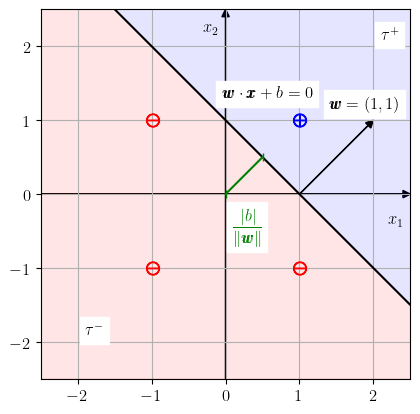
\includegraphics[width=0.7\textwidth]{./cap_perceptron/dados/fig_class_e/main}
  \caption{Interpretação geométrica do perceptron aplicado ao problema de classificação relacionado à operação lógica $\land$ (e-lógico).}
  \label{fig:class_e}
\end{figure}

\subsubsection{Algoritmo de treinamento: perceptron}
[[tag:construcao]]

O \hl{algoritmo de treinamento perceptron permite calibrar os pesos de um neurônio para fazer a classificação de dados linearmente separáveis}. Trata-se de um algoritmo para o \hl{\emph{treinamento supervisionado}} de um neurônio, i.e. \hl{a calibração dos pesos é feita com base em um dado \emph{conjunto de amostras de treinamento}}.

Seja dado um \emph{conjunto de treinamento} $\{\pmb{x}^{(s)},y^{(s)}\}_{s=1}^{n_s}$, onde $n_s$ é o número de amostras. O algoritmo consiste no seguinte:
\begin{enumerate}
\item $\pmb{w} \leftarrow\pmb{0}$, $b \leftarrow 0$.
\item Para $e \leftarrow 1,\dotsc, n_e$:
  \begin{enumerate}
  \item Para $s \leftarrow 1,\dotsc, n_s$:
    \begin{enumerate}
    \item Se $y^{(s)}\mathcal{N}\left(\pmb{x}^{(s)}\right) \leq 0$:
      \begin{enumerate}
      \item $\pmb{w} \leftarrow \pmb{w}+y^{(s)}\pmb{x}^{(s)}$
      \item $b \leftarrow b + y^{(s)}$
      \end{enumerate}
    \end{enumerate}
  \end{enumerate}
\end{enumerate}
onde, $n_e$ é um dado número de épocas\footnote{Número de vezes que as amostrar serão percorridas para realizar a correção dos pesos.}.

% \lstinputlisting[caption=perceptron\_train.py, label=cap_perceptron_sec_unit:cod:perceptron_train]{./cap_perceptron/dados/py_perceptron_train/main.py}
\begin{lstlisting}
import torch

# modelo

class Perceptron(torch.nn.Module):
    def __init__(self):
        super().__init__()
        self.linear = torch.nn.Linear(2,1)

    def forward(self, x):
        z =  self.linear(x)
        y = torch.sign(z)
        return y

model = Perceptron()
with torch.no_grad():
    W = model.linear.weight
    b = model.linear.bias

# dados de treinamento
X_train = torch.tensor([[1., 1.],
                  [1., -1.],
                  [-1., 1.],
                  [-1., -1.]])
y_train = torch.tensor([1., -1., -1., -1.]).reshape(-1,1)

## número de amostras
ns = y_train.size(0)

print("\nDados de treinamento")
print("X_train =")
print(X_train)
print("y_train = ")
print(y_train)

# treinamento

## num max épocas
nepochs = 100

for epoch in range(nepochs):

    # update
    not_updated = True
    for s in range(ns):
        y_est = model(X_train[s:s+1,:])
        if (y_est*y_train[s] <= 0.):
            with torch.no_grad():
                W += y_train[s]*X_train[s,:]
                b += y_train[s]
                not_updated = False

    if (not_updated):
        print('Training ended.')
        break


# verificação
print(f'W =\n{W}')
print(f'b =\n{b}')
y = model(X_train)
print(f'y =\n{y}')
\end{lstlisting}

\subsection{Problema de regressão}\label{cap_perceptron_sec_unit:ssec:regr}
[[tag:construcao]]

Vamos \hl{treinar um perceptron para resolver o problema de regressão linear} para os seguintes dados

\begin{center}
  \begin{tabular}{l|ll}
    s & $x^{(s)}$ & $y^{(s)}$\\\hline
    1 & 0.5 & 1.2\\
    2 & 1.0 & 2.1\\
    3 & 1.5 & 2.6\\
    4 & 2.0 & 3.6\\\hline
  \end{tabular}
\end{center}

\subsubsection{Modelo}
[[tag:construcao]]

Vamos determinar o perceptron\footnote{Escolhendo $f(z)=z$ como função de ativação.}
\begin{equation}\label{eq:percep_regr}
  \tilde{y} = \mathcal{N}(x; (w, b)) = wx + b
\end{equation}
que melhor se ajusta a este conjunto de dados $\left\{(x^{(s)}, y^{(s)})\right\}_{s=1}^{n_s}$, $n_s=4$.

\subsubsection{Treinamento}
[[tag:construcao]]

A \hl{ideia é que o perceptron seja tal que minimize o erro quadrático médio (MSE, do inglês, \textit{Mean Squared Error})}, i.e.
\begin{equation}\label{eq_percep:regr_prob}\hleq
  \min_{w,b}\frac{1}{n_s}\sum_{s=1}^{n_s}\left(\tilde{y}^{(s)}-y^{(s)}\right)^2
\end{equation}
Vamos denotar a \hl{\emph{função erro}} (em inglês, \textit{loss function}) por
\begin{align}\label{eq:eqm}
  \varepsilon(w,b) &:= \frac{1}{n_s}\sum_{s=1}^{n_s}\left(\tilde{y}^{(s)}-y^{(s)}\right)^2\\
                   &= \frac{1}{n_s}\sum_{s=1}^{n_s}\left(wx^{(s)}+b-y^{(s)}\right)^2
\end{align}

Observamos que o problema \eqref{eq_percep:regr_prob} é equivalente a um problema linear de \href{https://notaspedrok.com.br/notas/MatematicaNumerica/cap_ajuste_sec_prob_lin.html}{mínimos quadrados}. A solução é obtida resolvendo-se a equação normal\footnote{Consulte o Exercício \ref{exer_percep:sol_mq}.}
\begin{equation}\label{eq_percep:sol_mq}
  M^TM\pmb{c} = M^T\pmb{y},
\end{equation}
onde $\pmb{c} = (w, p)$ é o vetor dos parâmetros a determinar e $M$ é a matriz $n_s\times 2$ dada por
\begin{equation}
  M =
  \begin{bmatrix}
    \pmb{x} & \pmb{1}
  \end{bmatrix}
\end{equation}

\subsubsection{Implementação}
[[tag:construcao]]

% lstinputlisting[caption=perceptron\_mq.py, label=cap_perceptron_sec_unit:cod:perceptron_mq]{./cap_perceptron/dados/py_perceptron_mq/main.py}
\begin{lstlisting}[caption=perceptron\_mq.py, label=cap_perceptron_sec_unit:cod:perceptron_mq]
import torch

# modelo

class Perceptron(torch.nn.Module):
    def __init__(self):
        super().__init__()
        self.linear = torch.nn.Linear(1,1)

    def forward(self, x):
        z =  self.linear(x)
        return z

model = Perceptron()
with torch.no_grad():
    W = model.linear.weight
    b = model.linear.bias

# dados de treinamento
X_train = torch.tensor([0.5,
                        1.0,
                        1.5,
                        2.0]).reshape(-1,1)
y_train = torch.tensor([1.2,
                        2.1,
                        2.6,
                        3.6]).reshape(-1,1)

## número de amostras
ns = y_train.size(0)

print("\nDados de treinamento")
print("X_train =")
print(X_train)
print("y_train = ")
print(y_train)

# treinamento

## matriz
M = torch.cat((X_train,
               torch.ones((ns,1))), dim=1)
## solucão M.Q.
c = torch.linalg.lstsq(M, y_train)[0]
with torch.no_grad():
    W = c[0]
    b = c[1]

# verificação
print(f'W =\n{W}')
print(f'b =\n{b}')
y = model(X_train)
print(f'y =\n{y}')
\end{lstlisting}

\subsubsection{Resultado}
[[tag:construcao]]

Nosso perceptron corresponde ao modelo
\begin{equation}
  \mathcal{N}(x; (w,b)) = wx + b
\end{equation}
com os pesos treinados $w = 1.54$ e $b = 0.45$. Ele corresponde à reta que melhor se ajusta ao conjunto de dados de $\left\{x^{(s)}, y^{(s)}\right\}$. Consulte a Figura \ref{fig:percep_mq}.

\begin{figure}[H]
  \centering
  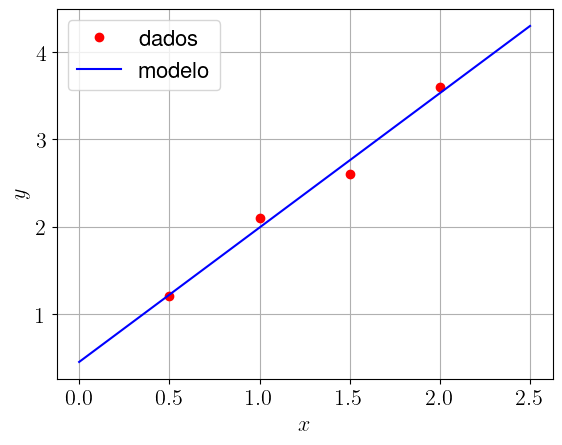
\includegraphics[width=0.7\textwidth]{./cap_perceptron/dados/fig_percep_mq/main}
  \caption{Interpretação geométrica do perceptron aplicado ao problema de regressão linear.}
  \label{fig:percep_mq}
\end{figure}

\subsection{Exercícios}
[[tag:construcao]]

\begin{exer}
  Crie um Perceptron que emule a operação lógica do $\lor$ (\texttt{ou-lógico}).
  \begin{center}
    \begin{tabular}{cc|c}
      $A_1$ & $A_2$ & $A_1\lor A_2$\\\hline
      V & V & V\\
      V & F & V\\
      F & V & V\\
      F & F & F\\\hline
    \end{tabular}
  \end{center}
\end{exer}

\begin{exer}
  Busque criar um Perceptron que emule a operação lógica do $\texttt{xor}$.
  \begin{center}
    \begin{tabular}{cc|c}
      $A_1$ & $A_2$ & $A_1\texttt{ xor }A_2$\\\hline
      V & V & F\\
      V & F & V\\
      F & V & V\\
      F & F & F\\\hline
    \end{tabular}
  \end{center}
  É possível? Justifique sua resposta.
\end{exer}

\begin{exer}\label{exer:eqm_convexa}
  Assumindo o modelo de neurônio \eqref{eq:percep_regr}, mostre que \eqref{eq:eqm} é função convexa.
\end{exer}
\begin{resp}
  Dica: verifique que sua matriz hessiana é positiva definida.
\end{resp}

\begin{exer}\label{exer_percep:sol_mq}
  Mostre que a solução do problema \eqref{eq_percep:regr_prob} é dada por \eqref{eq_percep:sol_mq}.
\end{exer}
\begin{resp}
  Dica: consulte a ligação \href{https://notaspedrok.com.br/notas/MatematicaNumerica/cap_ajuste_sec_prob_lin.html}{Notas de Aula: Matemática Numérica: 7.1 Problemas lineares}.
\end{resp}

\begin{exer}
  Crie um Perceptron com função de ativação $f(x)=\tanh(x)$ que melhor se ajuste ao seguinte conjunto de dados:
  \begin{center}
  \begin{tabular}{l|rr}
    s & $x^{(s)}$ & $y^{(s)}$\\\hline
    1 & -1,0 & -0,8 \\
    2 & -0,7 & -0,7 \\
    3 & -0,3 & -0,5 \\
    4 &  0,0 & -0,4 \\
    5 &  0,2 & -0,2 \\
    6 &  0,5 &  0,0 \\
    7 &  1,0 &  0,3 \\\hline
  \end{tabular}
\end{center}
\end{exer}

\section{Algoritmo de Treinamento}\label{cap_percepton_sec_train}
[[tag:construcao]]

Na seção anterior, desenvolvemos dois modelos de neurônios para problemas diferentes, um de classificação e outro de regressão. Em cada caso, utilizamos algoritmos de treinamento diferentes. Agora, vamos estudar algoritmos de treinamentos mais gerais\footnote{Aqui, vamos explorar apenas algoritmos de treinamento supervisionado.}, que podem ser aplicados a ambos os problemas.

Ao longo da seção, vamos considerar o \hl{\emph{modelo}} de neurônio
\begin{equation}
  \hleq \tilde{y} = \mathcal{N}\left(\pmb{x}; (\pmb{w}, b)\right) = f\underbrace{(\pmb{w}\cdot\pmb{x} + b)}_{z},
\end{equation}
com dada função de ativação $f:\mathbb{R}\to\mathbb{R}$, sendo os vetores de entrada $\pmb{x}$ e dos pesos $\pmb{w}$ de tamanho $n_{in}$. A pré-ativação do neurônio é denotada por
\begin{equation}
  z := \pmb{w}\cdot\pmb{x} + b
\end{equation}

\hl{Fornecido um \emph{conjunto de treinamento}} $\left\{\left(\pmb{x}^{(s)}, y^{(s)}\right)\right\}_1^{n_s}$, com $n_s$ amostras, \hl{o objetivo é calcular os parâmetros $(\pmb{w}, b)$ que minimizam a \emph{função erro quadrático médio}}
\begin{align}\label{eq:percep_mse}
  \hleq\varepsilon(\pmb{w}, b) &\hleq := \frac{1}{n_s}\sum_{s=1}^{n_s}\left(\tilde{y}^{(s)} - y^{(s)}\right)^2\\
                          &= \frac{1}{n_s}\sum_{s=1}^{n_s}\varepsilon^{(s)}
\end{align}
onde $\tilde{y}^{(s)} = \mathcal{N}\left(\pmb{x}^{(s)}; (\pmb{w}, b)\right)$ é o \emph{valor estimado} pelo modelo e $y^{(s)}$ é o \emph{valor esperado} para a $s$-ésima amostra. A função erro para a $s$-ésima amostra é
\begin{equation}\hleq
  \varepsilon^{(s)} := \left(\tilde{y}^{(s)} - y^{(s)}\right)^2.
\end{equation}

Ou seja, \hl{o treinamento consiste em resolver o seguinte \emph{problema de otimização}}
\begin{equation}\hleq
  \min_{(\pmb{w}, b)}\varepsilon(\pmb{w}, b)
\end{equation}

Para resolver este problema de otimização, vamos empregar o Método do Gradiente Descendente.

\subsection{Método do Gradiente Descendente}
[[tag:construcao]]

\hl{O \emph{Método do Gradiente Descendente} (GD, em inglês, \textit{Gradiente Descent Method}) é um }\href{https://notaspedrok.com.br/notas/MatematicaNumericaAvancada/cap_otimizacao_sec_minimi.html}{\hl{método de declive}}. Aplicado ao nosso modelo de Perceptron consiste no seguinte algoritmo:
\begin{enumerate}
\item $(\pmb{w}, b)$ aproximação inicial.
\item Para $e\leftarrow 1, \dotsc, n_e$:
  \begin{enumerate}
  \item $\displaystyle (\pmb{w}, b) \leftarrow (\pmb{w}, b) - l_r\frac{\p\varepsilon}{\p (\pmb{w}, b)}$
  \end{enumerate}
\end{enumerate}
onde, $n_e$ é o \hl{\emph{número de épocas}}, $l_r$ é uma dada \hl{\emph{taxa de aprendizagem} ($l_r$, do inglês, \textit{learning rate})} e o \hl{\emph{gradiente}} é
\begin{equation}\hleq
  \frac{\p\varepsilon}{\p (\pmb{w}, b)} := \left(\frac{\p\varepsilon}{\p w_1}, \dotsc, \frac{\p\varepsilon}{\p w_{n_{in}}}, \frac{\p\varepsilon}{\p b}\right)
\end{equation}

O cálculo do gradiente para os pesos $\pmb{w}$ pode ser feito como segue
\begin{align}
  \frac{\p\varepsilon}{\p \pmb{w}} &= \frac{\p}{\p\pmb{w}}\left[\frac{1}{n_s}\sum_{s=1}^{n_s}\varepsilon^{(s)}\right]\\
                                   &= \frac{1}{ns}\sum_{s=1}^{ns}\frac{\p\varepsilon^{(s)}}{\p\tilde{y}^{(s)}}\frac{\p\tilde{y}^{(s)}}{\p\pmb{w}}\\
  {\color{blue}\frac{\p\varepsilon}{\p \pmb{w}}} &{\color{blue}= \frac{1}{ns}\sum_{s=1}^{ns}\frac{\p\varepsilon^{(s)}}{\p\tilde{y}^{(s)}}\frac{\p\tilde{y}^{(s)}}{\p z^{(s)}}\frac{\p z^{(s)}}{\p\pmb{w}}}
\end{align}
Observando que
\begin{gather}
  \frac{\p\varepsilon^{(s)}}{\p\tilde{y}^{(s)}} = 2\left(\tilde{y}^{(s)} - y^{(s)}\right)\\
  \frac{\p\tilde{y}^{(s)}}{\p z^{(s)}} = f'\left(z^{(s)}\right)\\
  \frac{\p z^{(s)}}{\p\pmb{w}} = \pmb{x}^{(s)}
\end{gather}
obtemos
\begin{equation}
  \frac{\p\varepsilon}{\p \pmb{w}} = \frac{1}{n_s}\sum_{s=1}^{n_s}2\left(\tilde{y}^{(s)}-y^{(s)}\right)f'\left(z^{(s)}\right)\pmb{x}^{(s)}
\end{equation}
\begin{align}
  {\color{blue}\frac{\p\varepsilon}{\p b}} &{\color{blue}= \frac{1}{ns}\sum_{s=1}^{ns}\frac{\p\varepsilon^{(s)}}{\p\tilde{y}^{(s)}}\frac{\p\tilde{y}^{(s)}}{\p z^{(s)}}\frac{\p z^{(s)}}{\p b}}\\
  \frac{\p\varepsilon}{\p b} &= \frac{1}{n_s}\sum_{s=1}^{n_s}2\left(\tilde{y}^{(s)}-y^{(s)}\right)f'\left(z^{(s)}\right)\cdot 1
\end{align}

\subsubsection{Aplicação: Problema de Classificação}
[[tag:construcao]]

Na Subseção \ref{cap_perceptron_ssec_classic}, \hl{treinamos um Perceptron para o problema de classificação do e-lógico}. A função de ativação $f(x) = \sign(x)$ não é adequada para a aplicação do Método GD, pois $f'(x) \equiv 0$ para $x\neq 0$. Aqui, vamos usar
\begin{equation}
  f(x) = \tanh(x).
\end{equation}

% \lstinputlisting[caption=perceptron\_gd.py, label=cap_perceptron_sec_train:cod:perceptron_gd]{./cap_perceptron/dados/py_perceptron_gd/main.py}
\begin{lstlisting}[caption=perceptron\_gd.py, label=cap_perceptron_sec_train:cod:perceptron_gd]
import torch

# modelo

class Perceptron(torch.nn.Module):
    def __init__(self):
        super().__init__()
        self.linear = torch.nn.Linear(2,1)

    def forward(self, x):
        z =  self.linear(x)
        y = torch.tanh(z)
        return y

model = Perceptron()

# treinamento

## optimizador
optim = torch.optim.SGD(model.parameters(), lr=1e-1)

## função erro
loss_fun = torch.nn.MSELoss()

## dados de treinamento
X_train = torch.tensor([[1., 1.],
                  [1., -1.],
                  [-1., 1.],
                  [-1., -1.]])
y_train = torch.tensor([1., -1., -1., -1.]).reshape(-1,1)

print("\nDados de treinamento")
print("X_train =")
print(X_train)
print("y_train = ")
print(y_train)

## num max épocas
nepochs = 5000
tol = 1e-3

for epoch in range(nepochs):

    # forward
    y_est = model(X_train)

    # erro
    loss = loss_fun(y_est, y_train)

    print(f'{epoch}: {loss.item():.4e}')

    # critério de parada
    if (loss.item() < tol):
        break

    # backward
    optim.zero_grad()
    loss.backward()
    optim.step()


# verificação
y = model(X_train)
print(f'y_est = {y}')
\end{lstlisting}

\subsection{Método do Gradiente Estocástico}
[[tag:construcao]]

O \hl{\emph{Método do Gradiente Estocástico}} (SGD, do inglês, \textit{Stochastic Gradient Descent Method}) é um variação do Método GD. \hl{A ideia é atualizar os parâmetros do modelo com base no gradiente do erro de cada amostra (ou um subconjunto de amostras)}. A estocasticidade é obtida da randomização com que as amostras são escolhidas a cada época. O algoritmos consiste no seguinte:
\begin{enumerate}[1.]
\item \pmb{w}, b aproximações inicial.
\item Para $e\leftarrow 1,\dotsc, n_e$:
  \begin{enumerate}[1.1.]
  \item Para $s\leftarrow \texttt{random}(1,\dotsc, n_s)$:
    \begin{equation}
      (\pmb{w}, b) \leftarrow (\pmb{w}, b) - l_r\frac{\p\varepsilon^{(s)}}{\p(\pmb{w}, b)}
    \end{equation}
  \end{enumerate}
\end{enumerate}

\subsubsection{Aplicação: Problema de Classificação}
[[tag:construcao]]

% \lstinputlisting[caption=perceptron\_sgd.py, label=cap_perceptron_sec_train:cod:perceptron_sgd]{./cap_perceptron/dados/py_perceptron_sgd/main.py}
\begin{lstlisting}[caption=perceptron\_sgd.py, label=cap_perceptron_sec_train:cod:perceptron_sgd]
import torch
import numpy as np

# modelo

class Perceptron(torch.nn.Module):
    def __init__(self):
        super().__init__()
        self.linear = torch.nn.Linear(2,1)

    def forward(self, x):
        z =  self.linear(x)
        y = torch.tanh(z)
        return y

model = Perceptron()

# treinamento

## optimizador
optim = torch.optim.SGD(model.parameters(), lr=1e-1)

## função erro
loss_fun = torch.nn.MSELoss()

## dados de treinamento
X_train = torch.tensor([[1., 1.],
                  [1., -1.],
                  [-1., 1.],
                  [-1., -1.]])
y_train = torch.tensor([1., -1., -1., -1.]).reshape(-1,1)

## num de amostras
ns = y_train.size(0)

print("\nDados de treinamento")
print("X_train =")
print(X_train)
print("y_train = ")
print(y_train)

## num max épocas
nepochs = 5000
tol = 1e-3

for epoch in range(nepochs):

    # forward
    y_est = model(X_train)

    # erro
    loss = loss_fun(y_est, y_train)

    print(f'{epoch}: {loss.item():.4e}')

    # critério de parada
    if (loss.item() < tol):
        break

    # backward
    for s in torch.randperm(ns):
        loss_s = (y_est[s,:] - y_train[s,:])**2
        optim.zero_grad()
        loss_s.backward()
        optim.step()
        y_est = model(X_train)


# verificação
y = model(X_train)
print(f'y_est = {y}')
\end{lstlisting}


\subsection{Exercícios}
[[tag:construcao]]

\begin{exer}
  Calcule a derivada da função de ativação
  \begin{equation}
    f(x) = \tanh(x).
  \end{equation}
\end{exer}
\begin{resp}
  $(\tanh x)' = 1 - \tanh^2 x$
\end{resp}

\begin{exer}
  Crie um Perceptron para emular a operação lógica $\land$ (\texttt{e-lógico}). No treinamento, use como otimizador:
  \begin{enumerate}[a)]
  \item Método GD.
  \item Método SGD.
  \end{enumerate}
\end{exer}

\begin{exer}
  Crie um Perceptron para emular a operação lógica $\lor$ (\texttt{ou-lógico}). No treinamento, use como otimizador:
  \begin{enumerate}[a)]
  \item Método GD.
  \item Método SGD.
  \end{enumerate}
\end{exer}

\begin{exer}\label{cap_perceptron_sec_train:exer:ajuste}
  Crie um Perceptron que se ajuste ao seguinte conjunto de dados:
  \begin{center}
    \begin{tabular}{l|ll}
      s & $x^{(s)}$ & $y^{(s)}$\\\hline
      1 & 0.5 & 1.2\\
      2 & 1.0 & 2.1\\
      3 & 1.5 & 2.6\\
      4 & 2.0 & 3.6\\\hline
    \end{tabular}
  \end{center}
  No treinamento, use como otimizador:
  \begin{enumerate}[a)]
  \item Método GD.
  \item Método SGD.
  \end{enumerate}  
\end{exer}

%Este trabalho está licenciado sob a Licença Atribuição-CompartilhaIgual 4.0 Internacional Creative Commons. Para visualizar uma cópia desta licença, visite http://creativecommons.org/licenses/by-sa/4.0/deed.pt_BR ou mande uma carta para Creative Commons, PO Box 1866, Mountain View, CA 94042, USA.

\chapter{Perceptron Multicamadas}\label{cap_mlp}
\thispagestyle{fancy}

\section{Modelo MLP}\label{cap_mlp_sec_modelo}

\hl{Uma Perceptron Multicamadas (MLP, do inglês, \textit{Multilayer Perceptron}) é um tipo de Rede Neural Artificial formada por composições de camadas de perceptrons}. Consulte a Figura \ref{cap_mlp_sec_modelo}.

\begin{figure}[H]
  \centering
  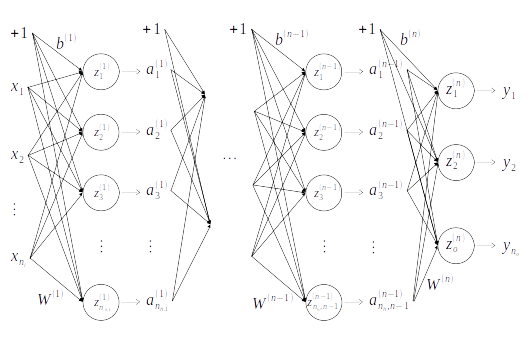
\includegraphics[width=\textwidth]{./cap_mlp/dados/fig_mlp/fig}
  \caption{Estrutura de uma rede do tipo Perceptron Multicamadas (MLP).}
  \label{fig:cap_mlp_sec_modelo:fig:mlp}
\end{figure}

\hl{Denotamos uma MLP de $n$ camadas por}
\begin{align}\hleq
  \pmb{y} = \mathcal{N}\left(\pmb{x}; \left(W^{(l)}, \pmb{b}^{(l)}, f^{(l)}\right)_{l=1}^{n}\right),
\end{align}
onde $\left(W^{(l)}, \pmb{b}^{(l)}, f^{(l)}\right)$ é a tripa de \emph{pesos}, \emph{\textit{biases}} e \emph{função de ativação} da $l$-ésima camada da rede, $l=1, 2, \dotsc, n$.

\hl{A saída da rede é calculada por iteradas composições das camadas}, i.e.
\begin{equation}\hleq
  \pmb{a}^{(l)} = f^{(l)}\underbrace{\left(W^{(l)}\pmb{a}^{(l-1)} + \pmb{b}^{(l-1)}\right)}_{\pmb{z}^{(l)}},
\end{equation}
para $l= 1, 2, \dotsc, n$, denotando $\pmb{a}^{(0)} := \pmb{x}$ e $\pmb{a}^{(n)} := \pmb{y}$.

\subsection{Treinamento}

Fornecido um \emph{conjunto de treinamento} $\{\pmb{x}^{(s)}, \pmb{y}^{(s)}\}_{s=1}^{n_s}$, com $n_s$ amostras, \hl{o treinamento da rede consiste em resolver o problema de minimização}
\begin{equation}\hleq
  \min_{(W,\pmb{b})}\varepsilon\left(\tilde{\pmb{y}}^{(s)}, \pmb{y}^{(s)}\right)
\end{equation}
onde $\varepsilon$ é uma dada \emph{função erro} (em inglês, \textit{loss function}) e $\tilde{\pmb{y}}^{(s)}$, $\pmb{y}^{(s)}$ são as saídas estimada e esperada da $l$-ésima amostra, respectivamente.

\hl{O problema de minimização pode ser resolvido por um }\href{https://notaspedrok.com.br/notas/MatematicaNumericaAvancada/cap\_otimizacao_sec_minimi.html}{\hl{Método de Declive}} e, de forma geral, consiste em:
\begin{enumerate}
\item $W, \pmb{b}$ aproximações iniciais.
\item Para $e\leftarrow 1, \dotsc, n_e$:
  \begin{enumerate}\hleq
  \item $\displaystyle (W, \pmb{b}) \leftarrow (W, \pmb{b}) - l_r\pmb{d}\left(\nabla_{W,\pmb{b}} \varepsilon\right)$
  \end{enumerate}
\end{enumerate}
onde, $n_e$ é o \emph{número de épocas}, $l_r$ é uma dada \emph{taxa de aprendizagem} (em inglês, \textit{learning rate})) e o vetor direção $\pmb{d} = \pmb{d}\left(\nabla_{W,\pmb{b}} \varepsilon\right)$, onde
\begin{equation}\hleq
  \nabla_{W,\pmb{b}} \varepsilon := \left(\frac{\p\varepsilon}{\p W}, \frac{\p\varepsilon}{\p\pmb{b}}\right).
\end{equation}

\hl{O cálculo dos gradientes pode ser feito \emph{de trás para frente}} (em inglês, \textit{backward}), i.e. para os pesos da última camada, temos
\begin{align}
  \hleq{\frac{\p\varepsilon}{\p W^{(n)}}} &\hleq{= \frac{\p\varepsilon}{\p\pmb{y}}\frac{\p\pmb{y}}{\p\pmb{z^{(n)}}}\frac{\p\pmb{z^{(n)}}}{\p W^{(n)}}},\\
                             &= \frac{\p\varepsilon}{\p\pmb{y}}f'\left(W^{(n)}\pmb{a}^{(n-1)}+\pmb{b}^{(n)}\right)\pmb{a}^{(n-1)}.
\end{align}
Para os pesos da penúltima, temos
\begin{align}
  \hleq{\frac{\p\varepsilon}{\p W^{(n-1)}}} &\hleq{= \frac{\p\varepsilon}{\p\pmb{y}}\frac{\p\pmb{y}}{\p\pmb{z^{(n)}}}\frac{\p\pmb{z^{(n)}}}{\p W^{(n-1)}}},\\
                                     &= \frac{\p\varepsilon}{\p\pmb{y}}f'\left(\pmb{z}^{(n)}\right)\frac{\p\pmb{z}^{(n)}}{\p\pmb{a}^{(n-1)}}\frac{\p\pmb{a}^{(n-1)}}{\p\pmb{z}^{(n-1)}}\frac{\p\pmb{z}^{(n-1)}}{\p W^{(n-1)}}\\
                                     &= \frac{\p\varepsilon}{\p\pmb{y}}f'\left(\pmb{z}^{(n)}\right)W^{(n)}f'\left(\pmb{z}^{(n-1)}\right)\pmb{a}^{(n-2)}
\end{align}
e assim, sucessivamente para as demais camadas da rede. \hl{Os gradientes em relação aos \textit{biases} podem ser analogamente calculados}.

\subsection{Aplicação: Problema de Classificação \texttt{XOR}}

Vamos desenvolver uma MLP que faça a operação $\texttt{xor}$ (ou exclusivo). I.e, receba como entrada dois valores lógicos $A_1$ e $A_2$ (V, verdadeiro ou F, falso) e forneça como saída o valor lógico $R = A_1 \texttt{xor} A_2$. Consultamos a seguinte tabela verdade:

\begin{center}
  \begin{tabular}{cc|c}
    $A_1$ & $A_2$ & $R$\\\hline
    V & V & F\\
    V & F & V\\
    F & V & V\\
    F & F & F\\\hline
  \end{tabular}
\end{center}

Assumindo $V = 1$ e $F = -1$, podemos modelar o problema tendo entradas $\pmb{x} = (x_1, x_2)$ e saída $y$ como na seguinte tabela:

\begin{center}
  \begin{tabular}{rr|r}
    $x_1$ & $x_2$ & $y$ \\\hline
    $1$ & $1$ & $-1$ \\
    $1$ & $-1$ & $1$ \\
    $-1$ & $1$ & $1$ \\
    $-1$ & $-1$ & $-1$ \\\hline
  \end{tabular}
\end{center}

\subsubsection{Modelo}

Vamos usar uma MLP de estrutura $2-2-1$ e com funções de ativação $f^{(1)}(\pmb{x}) = \tanh(\pmb{x})$ e $f^{(2)}(\pmb{x}) = id(\pmb{x})$. Ou seja, nossa rede tem duas entradas, uma \emph{camada escondida} com 2 unidades (função de ativação tangente hiperbólica) e uma camada de saída com uma unidade (função de ativação identidade).

\subsubsection{Treinamento}

Para o treinamento, vamos usar a função \hl{\emph{erro quadrático médio}} (em inglês, \textit{mean squared error})
\begin{equation}\hleq
  \varepsilon := \frac{1}{n_s}\sum_{s=1}^{n_s}\left|\tilde{y}^{(s)} - y^{(s)}\right|^2,
\end{equation}
onde os valores estimados $\tilde{y}^{(s)} = \mathcal{N}\left(\pmb{x}^{(s)}\right)$ e $\left\{\pmb{x}^{(s)}, y^{(s)}\right\}_{s=1}^{n_s}$, $n_s=4$, conforme na tabela acima.

\subsubsection{Implementação}

O seguinte código implementa a MLP e usa o \hl{Método do Gradiente Descendente (DG) no algoritmo de treinamento}.

% \lstinputlisting[caption=mlp\_xor.py, label=cap_mlp_sec_modelo:cod:mlp_xor]{./cap_mlp/dados/py_mlp_xor/main.py}
\begin{lstlisting}[caption=mlp\_xor.py, label=cap_mlp_sec_modelo:cod:mlp_xor]
import torch

# modelo

model = torch.nn.Sequential(
    torch.nn.Linear(2,2),
    torch.nn.Tanh(),
    torch.nn.Linear(2,1)
    )

# treinamento

## optimizador
optim = torch.optim.SGD(model.parameters(), lr=1e-2)

## função erro
loss_fun = torch.nn.MSELoss()

## dados de treinamento
X_train = torch.tensor([[1., 1.],
                  [1., -1.],
                  [-1., 1.],
                  [-1., -1.]])
y_train = torch.tensor([-1., 1., 1., -1.]).reshape(-1,1)

print("\nDados de treinamento")
print("X_train =")
print(X_train)
print("y_train = ")
print(y_train)

## num max épocas
nepochs = 5000
tol = 1e-3

for epoch in range(nepochs):

    # forward
    y_est = model(X_train)

    # erro
    loss = loss_fun(y_est, y_train)

    print(f'{epoch}: {loss.item():.4e}')

    # critério de parada
    if (loss.item() < tol):
        break

    # backward
    optim.zero_grad()
    loss.backward()
    optim.step()


# verificação
y = model(X_train)
print(f'y_est = {y}')
\end{lstlisting}

\subsection{Exercícios}

[[tag::construcao]]

\section{Aplicação: Problema de Classificação Binário}\label{cap_mlp_sec_classbin}

Vamos estudar uma aplicação de redes neurais artificiais em um problema de classificação binária não linear.

\subsection{Dados}

Vamos desenvolver uma rede do tipo Perceptron Multicamadas (MLP) para a classificação binária de pontos, com base nos seguintes dados.

\begin{lstlisting}
from sklearn.datasets import make_circles
import matplotlib.pyplot as plt

plt.rcParams.update({
     "text.usetex": True,
     "font.family": "serif",
     "font.size": 14
     })

# data
print('data')
n_samples = 1000
print(f'n_samples = {n_samples}')
# X = points, y = labels
X, y = make_circles(n_samples,
                    noise=0.03, # add noise
                    random_state=42) # random seed

fig = plt.figure()
ax = fig.add_subplot()
ax.scatter(X[:,0], X[:,1], c=y, cmap=plt.cm.coolwarm)
ax.grid()
ax.set_xlabel('$x_1$')
ax.set_ylabel('$x_2$')
plt.show()
\end{lstlisting}

\begin{figure}[H]
  \centering
  \includegraphics[width=0.8\textwidth]{./cap_mlp/dados/fig_classbin/fig}
  \caption{Dados para a o problema de classificação binária não linear.}
  \label{cap_mlp_sec_classbin:fig:dados}
\end{figure}

\subsection{Modelo}

Vamos usar uma MLP de estrutura 2-10-1, com função de ativação
\begin{equation}
  \elu(x) = \left\{
    \begin{array}{ll}
      x &, x > 0\\
      \alpha\left(e^x - 1\right) &, x \leq 0
    \end{array}
\right.
\end{equation}
na camada escondida e
\begin{equation}
  \sigmoid(x) = \frac{1}{1 + e^x}
\end{equation}
na saída da rede.

Para o treinamento e teste, vamos randomicamente separar os dados em um conjunto de treinamento $\{\pmb{x}_{\text{train}}^{(k)}, y_{\text{train}}^{(k)}\}_{k=1}^{n_{\text{train}}}$ e um conjunto de teste $\{\pmb{x}_{\text{test}}^{(k)}, y_{\text{test}}^{(k)}\}_{k=1}^{n_{\text{test}}}$, com $y=0$ para os pontos azuis e $y=1$ para os pontos vermelhos.

\subsection{Treinamento e Teste}

\begin{lstlisting}[caption=mlp\_classbin.py, label=cap_mlp_sec_classbin:cod:classbin]
import torch
from sklearn.datasets import make_circles
from sklearn.model_selection import train_test_split
import matplotlib.pyplot as plt

# data
print('data')
n_samples = 1000
print(f'n_samples = {n_samples}')
# X = points, y = labels
X, y = make_circles(n_samples,
                    noise=0.03, # add noise
                    random_state=42) # random seed

## numpy -> torch
X = torch.from_numpy(X).type(torch.float)
y = torch.from_numpy(y).type(torch.float).reshape(-1,1)

## split into train and test datasets
print('Data: train and test sets')
X_train, X_test, y_train, y_test = train_test_split(X,
                                                    y,
                                                    test_size=0.2,
                                                    random_state=42)
print(f'n_train = {len(X_train)}')
print(f'n_test = {len(X_test)}')
plt.close()
plt.scatter(X_train[:,0], X_train[:,1], c=y_train,
            marker='o', cmap=plt.cm.coolwarm, alpha=0.3)
plt.scatter(X_test[:,0], X_test[:,1], c=y_test,
            marker='*', cmap=plt.cm.coolwarm)
plt.show()

# model
model = torch.nn.Sequential(
    torch.nn.Linear(2, 10),
    torch.nn.ELU(),
    torch.nn.Linear(10, 1),
    torch.nn.Sigmoid()
    )

# loss fun
loss_fun = torch.nn.BCELoss()

# optimizer
optimizer = torch.optim.SGD(model.parameters(),
                            lr = 1e-1)

# evaluation metric
def accuracy_fun(y_pred, y_exp):
    correct = torch.eq(y_pred, y_exp).sum().item()
    acc = correct/len(y_exp) * 100
    return acc

# train
n_epochs = 10000
n_out = 100

for epoch in range(n_epochs):
    model.train()

    y_pred = model(X_train)

    loss = loss_fun(y_pred, y_train)

    acc = accuracy_fun(torch.round(y_pred),
                       y_train)

    optimizer.zero_grad()
    loss.backward()
    optimizer.step()

    model.eval()

    #testing
    if ((epoch+1) % n_out == 0):
        with torch.inference_mode():
            y_pred_test = model(X_test)
            loss_test = loss_fun(y_pred_test,
                                 y_test)
            acc_test = accuracy_fun(torch.round(y_pred_test),
                                    y_test)

        print(f'{epoch+1}: loss = {loss:.5e}, accuracy = {acc:.2f}%')
        print(f'\ttest: loss = {loss:.5e}, accuracy = {acc:.2f}%\n')
\end{lstlisting}

\subsection{Verificação}

Para a verificação, testamos o modelo em uma malha uniforme de $100\times 100$ pontos no domínio $[-1, 1]^2$. Consulte a Figure \ref{cap_mlp_sec_classbin:fig:result}.

\begin{figure}[H]
  \centering
  \includegraphics[width=0.8\textwidth]{./cap_mlp/dados/fig_classbin_result/fig}
  \caption{Verificação do modelo de classificação binária.}
  \label{cap_mlp_sec_classbin:fig:result}
\end{figure}


\begin{lstlisting}
# malha de pontos
xx = torch.linspace(-1.1, 1.1, 100)
Xg, Yg = torch.meshgrid(xx, xx)

# valores estimados
Zg = torch.empty_like(Xg)
for i,xg in enumerate(xx):
    for j,yg in enumerate(xx):
        z = model(torch.tensor([[xg, yg]])).detach()
        Zg[i, j] = torch.round(z)

# visualização
fig = plt.figure()
ax = fig.add_subplot()
ax.contourf(Xg, Yg, Zg, levels=2, cmap=plt.cm.coolwarm, alpha=0.5)
ax.scatter(X[:,0], X[:,1], c=y, cmap=plt.cm.coolwarm)
plt.show()
\end{lstlisting}

\subsection{Exercícios}

[[tag:construcao]]


\section{Aplicação: Aproximação de Funções}\label{cap_mlp_sec_apfun}

\hl{Redes Perceptron Multicamadas (MLP) são aproximadoras universais}. Nesta seção, vamos aplicá-las na aproximação de funções uni- e bidimensionais.

\subsection{Função unidimensional}

Vamos criar uma MLP para aproximar a função gaussiana
\begin{equation}
  y = e^{-x^2},
\end{equation}
para $x\in [-1,1]$.

% \lstinputlisting[caption=mlp\_gaussiana\_1d.py, label=cap_mlp_sec_modelo:cod:mlp_gaussiana_1d]{./cap_mlp/dados/py_mlp_gaussiana_1d/main.py}
\begin{lstlisting}
import torch
import matplotlib.pyplot as plt

# modelo

model = torch.nn.Sequential(
    torch.nn.Linear(1,25),
    torch.nn.Tanh(),
    torch.nn.Linear(25,1)
    )

# treinamento

## fun obj
fobj = lambda x: torch.exp(-x**2)
a = -1.
b = 1.

## optimizador
optim = torch.optim.SGD(model.parameters(),
                        lr=1e-2, momentum=0.9)

## função erro
loss_fun = torch.nn.MSELoss()

## num de amostras por época
ns = 100
## num max épocas
nepochs = 5000
## tolerância
tol = 1e-5

for epoch in range(nepochs):

    # amostras
    X_train = (a - b) * torch.rand((ns,1)) + b
    y_train = fobj(X_train)
    
    # forward
    y_est = model(X_train)

    # erro
    loss = loss_fun(y_est, y_train)

    print(f'{epoch}: {loss.item():.4e}')

    # critério de parada
    if (loss.item() < tol):
        break

    # backward
    optim.zero_grad()
    loss.backward()
    optim.step()


# verificação
fig = plt.figure()
ax = fig.add_subplot()

x = torch.linspace(a, b,
                   steps=50).reshape(-1,1)

y_esp = fobj(x)
ax.plot(x, y_esp, label='fobj')

y_est = model(x)
ax.plot(x, y_est.detach(), label='model')

ax.legend()
ax.grid()
ax.set_xlabel('x')
ax.set_ylabel('y')
plt.show()
\end{lstlisting}

\subsection{Função bidimensional}

Vamos criar uma MLP para aproximar a função gaussiana
\begin{equation}
  y = e^{-(x_1^2 + x_2^2)},
\end{equation}
para $\pmb{x} = (x_1, x_2)\in [-1,1]^2$.

% \lstinputlisting[caption=mlp\_gaussiana\_2d.py, label=cap_mlp_sec_modelo:cod:mlp_gaussiana_2d]{./cap_mlp/dados/py_mlp_gaussiana_2d/main.py}
\begin{lstlisting}
import torch
import matplotlib.pyplot as plt

# modelo

model = torch.nn.Sequential(
    torch.nn.Linear(2,50),
    torch.nn.Tanh(),
    torch.nn.Linear(50,25),
    torch.nn.Tanh(),
    torch.nn.Linear(25,5),
    torch.nn.Tanh(),
    torch.nn.Linear(5,1)
    )

# treinamento

## fun obj
a = -1.
b = 1.
def fobj(x):
    y = torch.exp(-x[:,0]**2 - x[:,1]**2)
    return y.reshape(-1,1)

## optimizador
optim = torch.optim.SGD(model.parameters(),
                        lr=1e-1, momentum=0.9)

## função erro
loss_fun = torch.nn.MSELoss()

## num de amostras por eixo por época
ns = 100
## num max épocas
nepochs = 5000
## tolerância
tol = 1e-5

for epoch in range(nepochs):

    # amostras
    x0 = (a - b) * torch.rand(ns) + b
    x1 = (a - b) * torch.rand(ns) + b
    X0, X1 = torch.meshgrid(x0, x1)
    X_train = torch.cat((X0.reshape(-1,1),
                         X1.reshape(-1,1)),
                        dim=1)
    y_train = fobj(X_train)
    
    # forward
    y_est = model(X_train)

    # erro
    loss = loss_fun(y_est, y_train)

    print(f'{epoch}: {loss.item():.4e}')

    # critério de parada
    if (loss.item() < tol):
        break

    # backward
    optim.zero_grad()
    loss.backward()
    optim.step()


# verificação
fig = plt.figure()
ax = fig.add_subplot()

n = 50
x0 = torch.linspace(a, b, steps=n)
x1 = torch.linspace(a, b, steps=n)
X0, X1 = torch.meshgrid(x0, x1)
X = torch.cat((X0.reshape(-1,1),
               X1.reshape(-1,1)),
              dim=1)

y_esp = fobj(X)
Y = y_esp.reshape((n,n))
levels = torch.linspace(0., 1., 10)
c = ax.contour(X0, X1, Y, levels=levels, colors='white')
ax.clabel(c)

y_est = model(X)
Y = y_est.reshape((n,n))
ax.contourf(X0, X1, Y.detach(), levels=levels)

ax.grid()
ax.set_xlabel('x_1')
ax.set_ylabel('x_2')
plt.show()
\end{lstlisting}

\subsection{Exercícios}

[[tag::construcao]]

\section{Aplicação: Equação de Laplace}\label{cap_mlp_sec_eqlaplace}

Vamos criar uma MLP para resolver
\begin{subequations}
  \begin{align}
    -\Delta u &= 0,\quad \pmb{x}\in D = (0, 1)^2,\\
    u &= 0,\quad \pmb{x}\in\p D.
  \end{align}
\end{subequations}

Como exemplo, vamos considerar um problema com solução manufaturada
\begin{equation}
  u(\pmb{x}) = x_1(1-x_1) - x_2(1-x_2).
\end{equation}

\subsection{Diferenças Finitas}

% \lstinputlisting[caption=mlp\_eqlaplace.py, label=cap_mlp_sec_modelo:cod:mlp_eqlaplace]{./cap_mlp/dados/py_mlp_eqlaplace/main.py}
\begin{lstlisting}[caption=mlp\_eqlaplace\_df.py, label=cap_mlp_sec_modelo:cod:mlp_eqlaplace_df]
import torch
import matplotlib.pyplot as plt
import random
import numpy as np

# modelo
model = torch.nn.Sequential(
    torch.nn.Linear(2,50),
    torch.nn.Tanh(),
    torch.nn.Linear(50,10),
    torch.nn.Tanh(),
    torch.nn.Linear(10,5),
    torch.nn.Tanh(),
    torch.nn.Linear(5,1)
)

# SGD - (Stochastic) Gradient Descent
optim = torch.optim.SGD(model.parameters(),
                        lr = 1e-3,
                        momentum = 0.9,
                        dampening = 0.)

# Solução esperada
def u(x, y):
    return a*x*(1-x) - a*y*(1-y)


def laplace_loss(X, U, h2, n, uc=u, p=1.):
    # num de amostras
    nc = 2*n + 2*(n-2)
    ni = n**2 - nc

    # loss interno
    lin = 0.
    for i in range(1,n-1):
      for j in range(1,n-1):
        s = j + i*n
        l = (U[s-n, 0] - 2 * U[s, 0] + U[s+n, 0])/h2 # x
        l += (U[s-1, 0] - 2 * U[s, 0] + U[s+1, 0])/h2 # y
        lin += l**2
    lin /= ni 

    # loss contorno
    lc = 0.
    # 0 <= x <= 1 e y == 0
    for i in range(n):
        s = i*n
        x = M[s,0]
        y = M[s,1]
        lc += (U[s,0] - uc(x,y))**2
    # 0 <= x <= 1 e y == 1
    for i in range(n):
        s = n-1 + i*n
        x = M[s,0]
        y = M[s,1]
        lc += (U[s,0] - uc(x,y))**2
    # 0 == x e 0 < y < 1
    for j in range(1, n-1):
        s = j
        x = M[s,0]
        y = M[s,1]
        lc += (U[s,0] - uc(x,y))**2
    # 1 == x e 0 < y < 1
    for j in range(1, n-1):
        s = j + n*(n-1)
        x = M[s,0]
        y = M[s,1]
        lc += (U[s,0] - uc(x,y))**2
    lc *= p/nc
    
    loss = lin + lc
    return loss

    
# dados do problema

# collocation points
a = 1
n = 11
ns = n**2
h = 1./(n-1)
h2 = h**2

# malha
x = torch.linspace(0, 1, n)
y = torch.linspace(0, 1, n)

M = torch.empty((ns, 2))
s = 0
for i, xx in enumerate(x):
  for j, yy in enumerate(y):
    M[s,0] = xx
    M[s,1] = yy
    s += 1

# gráfico
X, Y = np.meshgrid(x, y)
U_esp = u(X, Y)

# training
nepochs = 10000
nout_loss = 100
nout_plot = 500

for epoch in range(nepochs):

    # forward
    U_est = model(M)

    # loss function
    loss = laplace_loss(M, U_est, h2, n, u, p=10.)

    if ((epoch % nout_loss) == 0):
        print(f'{epoch}: loss = {loss.item():.4e}')
    
    # output current solution
    if ((epoch) % nout_plot == 0):
        # verificação
        fig = plt.figure()
        ax = fig.add_subplot()

        ns = 50
        x1 = torch.linspace(0., 1., ns)
        x2 = torch.linspace(0., 1., ns)
        X1, X2 = torch.meshgrid(x1, x2)
        # exact
        Z_esp = torch.empty_like(X1)
        for i,x in enumerate(x1):
            for j,y in enumerate(x2):
                Z_esp[i,j] = u(x, y)
        c = ax.contour(X1, X2, Z_esp, levels=10, colors='white')
        ax.clabel(c)

        X_plot = torch.cat((X1.reshape(-1,1),
                            X2.reshape(-1,1)), dim=1)
        Z_est = model(X_plot)
        Z_est = Z_est.reshape((ns,ns))
        cf = ax.contourf(X1, X2, Z_est.detach(), levels=10, cmap='coolwarm')
        plt.colorbar(cf)
        
        ax.grid()
        ax.set_xlabel('$x_1$')
        ax.set_ylabel('$x_2$')
        plt.show()        

    # backward
    optim.zero_grad()
    loss.backward()
    optim.step()
\end{lstlisting}

\subsection{Autograd}

\begin{lstlisting}[caption=mlp\_eqlaplace\_ag.py, label=cap_mlp_sec_modelo:cod:mlp_eqlaplace_ag]
import torch
import matplotlib.pyplot as plt
import random
import numpy as np

# modelo
model = torch.nn.Sequential(
    torch.nn.Linear(2,50),
    torch.nn.Tanh(),
    torch.nn.Linear(50,10),
    torch.nn.Tanh(),
    torch.nn.Linear(10,5),
    torch.nn.Tanh(),
    torch.nn.Linear(5,1)
)

# SGD - (Stochastic) Gradient Descent
optim = torch.optim.SGD(model.parameters(),
                        lr = 1e-3,
                        momentum = 0.9,
                        dampening = 0.)

# Solução esperada
def u(x, y):
    return a*x*(1-x) - a*y*(1-y)


def laplace_loss(X, U, h2, n, uc=u, p=1.):
    # num de amostras
    nc = 2*n + 2*(n-2)
    ni = n**2 - nc

    # loss interno
    lin = 0.
    for i in range(1,n-1):
      for j in range(1,n-1):
        s = j + i*n
        x = X[s:s+1,:].detach()
        x.requires_grad = True
        u = model(x)
        grad_u = torch.autograd.grad(u, x,
                                     create_graph = True,
                                     retain_graph = True)[0]
        u_x = grad_u[0,0]
        u_y = grad_u[0,1]

        u_xx = torch.autograd.grad(u_x, x,
                                   create_graph = True,
                                   retain_graph = True)[0][0,0]
        u_yy = torch.autograd.grad(u_y, x,
                                   create_graph = True,
                                   retain_graph = True)[0][0,1]
        lin = torch.add(lin, (u_xx + u_yy)**2)
    lin /= ni 

    # loss contorno
    lc = 0.
    # 0 <= x <= 1 e y == 0
    for i in range(n):
        s = i*n
        x = M[s,0]
        y = M[s,1]
        lc += (U[s,0] - uc(x,y))**2
    # 0 <= x <= 1 e y == 1
    for i in range(n):
        s = n-1 + i*n
        x = M[s,0]
        y = M[s,1]
        lc += (U[s,0] - uc(x,y))**2
    # 0 == x e 0 < y < 1
    for j in range(1, n-1):
        s = j
        x = M[s,0]
        y = M[s,1]
        lc += (U[s,0] - uc(x,y))**2
    # 1 == x e 0 < y < 1
    for j in range(1, n-1):
        s = j + n*(n-1)
        x = M[s,0]
        y = M[s,1]
        lc += (U[s,0] - uc(x,y))**2
    lc *= p/nc
    
    loss = lin + lc
    return loss

    
# dados do problema

# collocation points
a = 1
n = 11
ns = n**2
h = 1./(n-1)
h2 = h**2

# malha
x = torch.linspace(0, 1, n)
y = torch.linspace(0, 1, n)

M = torch.empty((ns, 2))
s = 0
for i, xx in enumerate(x):
  for j, yy in enumerate(y):
    M[s,0] = xx
    M[s,1] = yy
    s += 1

# gráfico
X, Y = np.meshgrid(x, y)
U_esp = u(X, Y)

# training
nepochs = 10000
nout_loss = 100
nout_plot = 500

for epoch in range(nepochs):

    # forward
    U_est = model(M)

    # loss function
    loss = laplace_loss(M, U_est, h2, n, u, p=10.)

    if ((epoch % nout_loss) == 0):
        print(f'{epoch}: loss = {loss.item():.4e}')
    
    # output current solution
    if ((epoch) % nout_plot == 0):
        # verificação
        fig = plt.figure()
        ax = fig.add_subplot()

        ns = 50
        x1 = torch.linspace(0., 1., ns)
        x2 = torch.linspace(0., 1., ns)
        X1, X2 = torch.meshgrid(x1, x2)
        # exact
        Z_esp = torch.empty_like(X1)
        for i,x in enumerate(x1):
            for j,y in enumerate(x2):
                Z_esp[i,j] = u(x, y)
        c = ax.contour(X1, X2, Z_esp, levels=10, colors='white')
        ax.clabel(c)

        X_plot = torch.cat((X1.reshape(-1,1),
                            X2.reshape(-1,1)), dim=1)
        Z_est = model(X_plot)
        Z_est = Z_est.reshape((ns,ns))
        cf = ax.contourf(X1, X2, Z_est.detach(), levels=10, cmap='coolwarm')
        plt.colorbar(cf)
        
        ax.grid()
        ax.set_xlabel('$x_1$')
        ax.set_ylabel('$x_2$')
        plt.show()        

    # backward
    optim.zero_grad()
    loss.backward()
    optim.step()
\end{lstlisting}

\subsection{Exercícios}

[[tag::construcao]]


%resposta dos exercícios
\ifisbook
%Este trabalho está licenciado sob a Licença Atribuição-CompartilhaIgual 4.0 Internacional Creative Commons. Para visualizar uma cópia desta licença, visite http://creativecommons.org/licenses/by-sa/4.0/ ou mande uma carta para Creative Commons, PO Box 1866, Mountain View, CA 94042, USA.

\chapter*{Resposta dos Exercícios}\label{cap_respostas}
\addcontentsline{toc}{chapter}{Respostas dos Exercícios}

\shipoutAnswer
\fi

%references
\nocite{*}
\bibliography{main}
\addcontentsline{toc}{chapter}{Referências Bibliográficas}

\ifisbook
\clearpage
\addcontentsline{toc}{chapter}{Índice Remissivo}
\printindex
\fi

\end{document}
